\documentclass{standalone}
\usepackage{tikz}
\usetikzlibrary{patterns, positioning}


\begin{document}
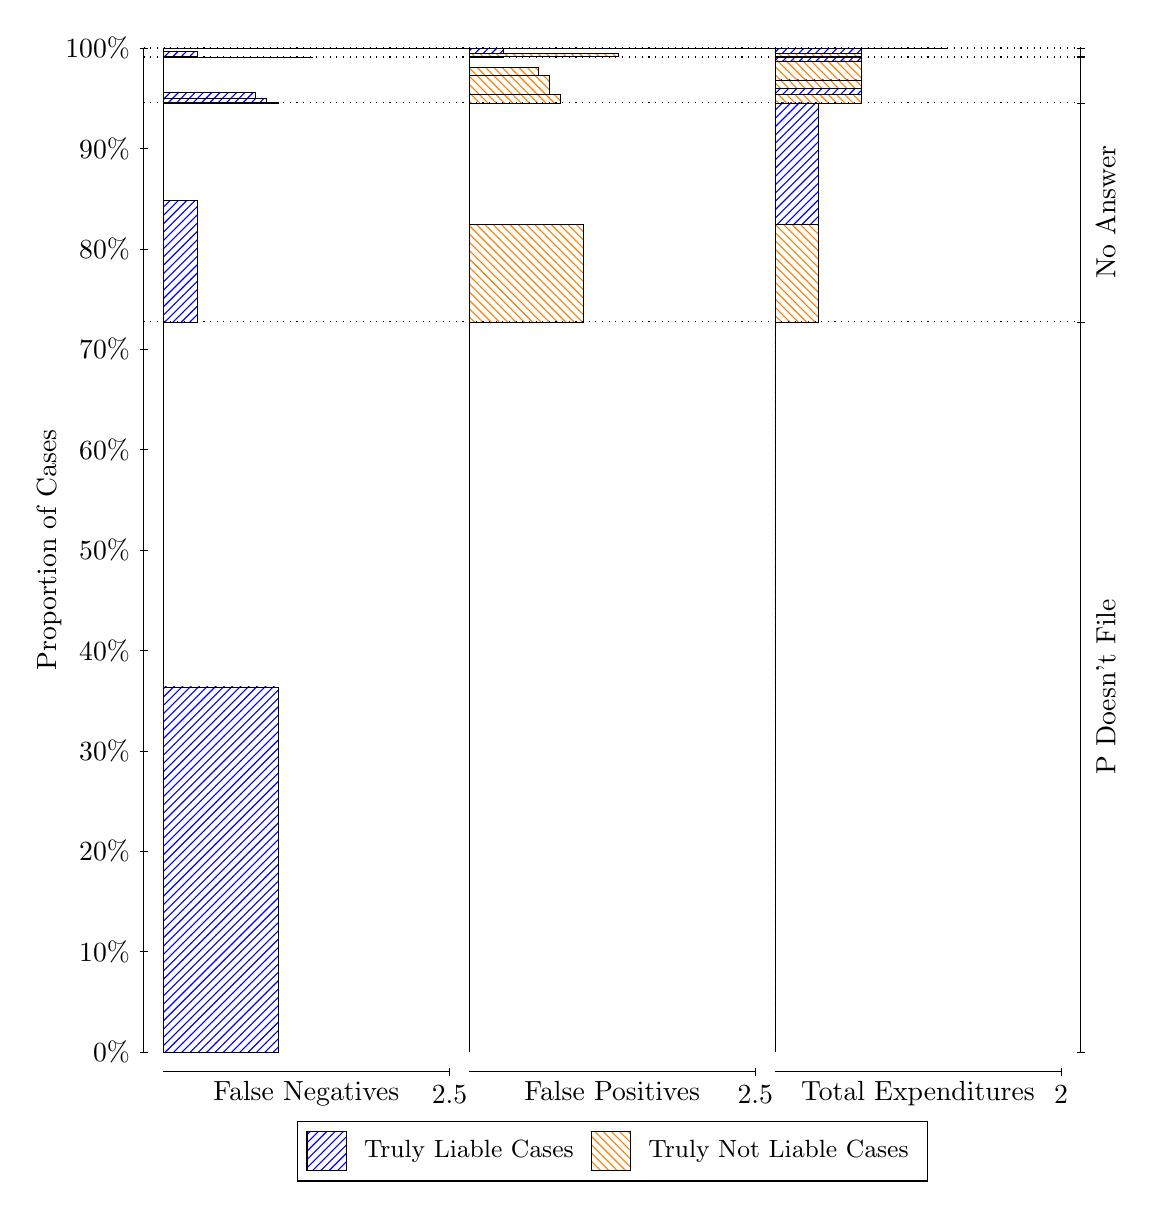
\begin{tikzpicture}
\draw[black, very thin] (1.5,1.75) -- (1.5,14.5);
\node[rotate=90, text=black, anchor=center] at (0.3, 8.125) {Proportion of Cases};
\draw[black, very thin] (1.45,1.75) -- (1.55,1.75);
\node[text=black, anchor=east] at (1.45, 1.75) {0\%};
\draw[black, very thin] (1.45,3.025) -- (1.55,3.025);
\node[text=black, anchor=east] at (1.45, 3.025) {10\%};
\draw[black, very thin] (1.45,4.3) -- (1.55,4.3);
\node[text=black, anchor=east] at (1.45, 4.3) {20\%};
\draw[black, very thin] (1.45,5.575) -- (1.55,5.575);
\node[text=black, anchor=east] at (1.45, 5.575) {30\%};
\draw[black, very thin] (1.45,6.85) -- (1.55,6.85);
\node[text=black, anchor=east] at (1.45, 6.85) {40\%};
\draw[black, very thin] (1.45,8.125) -- (1.55,8.125);
\node[text=black, anchor=east] at (1.45, 8.125) {50\%};
\draw[black, very thin] (1.45,9.4) -- (1.55,9.4);
\node[text=black, anchor=east] at (1.45, 9.4) {60\%};
\draw[black, very thin] (1.45,10.675) -- (1.55,10.675);
\node[text=black, anchor=east] at (1.45, 10.675) {70\%};
\draw[black, very thin] (1.45,11.95) -- (1.55,11.95);
\node[text=black, anchor=east] at (1.45, 11.95) {80\%};
\draw[black, very thin] (1.45,13.225) -- (1.55,13.225);
\node[text=black, anchor=east] at (1.45, 13.225) {90\%};
\draw[black, very thin] (1.45,14.5) -- (1.55,14.5);
\node[text=black, anchor=east] at (1.45, 14.5) {100\%};

\draw[black, very thin] (13.4,1.75) -- (13.4,14.5);
\draw[black, very thin] (13.35,1.75) -- (13.45,1.75);
\node[anchor=west] at (13.35, 1.75) {};
\draw[black, very thin] (13.35,11.023) -- (13.45,11.023);
\node[anchor=west] at (13.35, 11.023) {};
\draw[black, very thin] (13.35,13.803) -- (13.45,13.803);
\node[anchor=west] at (13.35, 13.803) {};
\draw[black, very thin] (13.35,14.381) -- (13.45,14.381);
\node[anchor=west] at (13.35, 14.381) {};
\draw[black, very thin] (13.35,14.397) -- (13.45,14.397);
\node[anchor=west] at (13.35, 14.397) {};
\draw[black, very thin] (13.35,14.5) -- (13.45,14.5);
\node[anchor=west] at (13.35, 14.5) {};
\draw[black, very thin] (13.35,14.5) -- (13.45,14.5);
\node[anchor=west] at (13.35, 14.5) {};
\draw[black, very thin] (13.35,14.5) -- (13.45,14.5);
\node[anchor=west] at (13.35, 14.5) {};

\draw[black, very thin, pattern color=blue, pattern=north east lines] (1.75,1.75) rectangle (3.2033,6.3863);
\draw[black, very thin, pattern color=orange, pattern=north west lines] (1.75,6.3863) rectangle (1.75,11.023);
\draw[black, very thin, pattern color=blue, pattern=north east lines] (1.75,11.023) rectangle (2.186,12.564);
\draw[black, very thin, pattern color=orange, pattern=north west lines] (1.75,12.564) rectangle (1.75,13.803);
\draw[black, very thin, pattern color=blue, pattern=north east lines] (1.75,13.803) rectangle (3.2033,13.811);
\draw[black, very thin, pattern color=blue, pattern=north east lines] (1.75,13.811) rectangle (3.058,13.856);
\draw[black, very thin, pattern color=blue, pattern=north east lines] (1.75,13.856) rectangle (2.9127,13.934);
\draw[black, very thin, pattern color=orange, pattern=north west lines] (1.75,13.934) rectangle (1.75,14.381);
\draw[black, very thin, pattern color=blue, pattern=north east lines] (1.75,14.381) rectangle (3.6393,14.383);
\draw[black, very thin, pattern color=orange, pattern=north west lines] (1.75,14.383) rectangle (1.75,14.397);
\draw[black, very thin, pattern color=blue, pattern=north east lines] (1.75,14.397) rectangle (2.186,14.46);
\draw[black, very thin, pattern color=orange, pattern=north west lines] (1.75,14.46) rectangle (1.75,14.5);
\draw[black, very thin, pattern color=blue, pattern=north east lines] (1.75,14.5) rectangle (5.8193,14.5);
\draw[black, very thin, pattern color=orange, pattern=north west lines] (1.75,14.5) rectangle (1.75,14.5);
\draw[black, very thin, pattern color=orange, pattern=north west lines] (1.75,14.5) rectangle (1.75,14.5);
\draw[black, very thin, pattern color=blue, pattern=north east lines] (1.75,14.5) rectangle (1.75,14.5);
\draw[black, very thin, pattern color=orange, pattern=north west lines] (5.6333,1.75) rectangle (5.6333,6.3864);
\draw[black, very thin, pattern color=blue, pattern=north east lines] (5.6333,6.3864) rectangle (5.6333,11.023);
\draw[black, very thin, pattern color=orange, pattern=north west lines] (5.6333,11.023) rectangle (7.0867,12.261);
\draw[black, very thin, pattern color=blue, pattern=north east lines] (5.6333,12.261) rectangle (5.6333,13.803);
\draw[black, very thin, pattern color=orange, pattern=north west lines] (5.6333,13.803) rectangle (6.796,13.909);
\draw[black, very thin, pattern color=orange, pattern=north west lines] (5.6333,13.909) rectangle (6.6507,14.151);
\draw[black, very thin, pattern color=orange, pattern=north west lines] (5.6333,14.151) rectangle (6.5053,14.25);
\draw[black, very thin, pattern color=blue, pattern=north east lines] (5.6333,14.25) rectangle (5.6333,14.381);
\draw[black, very thin, pattern color=orange, pattern=north west lines] (5.6333,14.381) rectangle (6.0693,14.394);
\draw[black, very thin, pattern color=blue, pattern=north east lines] (5.6333,14.394) rectangle (5.6333,14.397);
\draw[black, very thin, pattern color=orange, pattern=north west lines] (5.6333,14.397) rectangle (7.5227,14.436);
\draw[black, very thin, pattern color=blue, pattern=north east lines] (5.6333,14.436) rectangle (6.0693,14.5);
\draw[black, very thin, pattern color=orange, pattern=north west lines] (5.6333,14.5) rectangle (5.6333,14.5);
\draw[black, very thin, pattern color=blue, pattern=north east lines] (5.6333,14.5) rectangle (5.6333,14.5);
\draw[black, very thin, pattern color=orange, pattern=north west lines] (5.6333,14.5) rectangle (9.7027,14.5);
\draw[black, very thin, pattern color=blue, pattern=north east lines] (5.6333,14.5) rectangle (8.2493,14.5);
\draw[black, very thin, pattern color=orange, pattern=north west lines] (9.5167,1.75) rectangle (9.5167,6.3864);
\draw[black, very thin, pattern color=blue, pattern=north east lines] (9.5167,6.3864) rectangle (9.5167,11.023);
\draw[black, very thin, pattern color=orange, pattern=north west lines] (9.5167,11.023) rectangle (10.062,12.261);
\draw[black, very thin, pattern color=blue, pattern=north east lines] (9.5167,12.261) rectangle (10.062,13.803);
\draw[black, very thin, pattern color=orange, pattern=north west lines] (9.5167,13.803) rectangle (10.607,13.909);
\draw[black, very thin, pattern color=blue, pattern=north east lines] (9.5167,13.909) rectangle (10.607,13.987);
\draw[black, very thin, pattern color=orange, pattern=north west lines] (9.5167,13.987) rectangle (10.607,14.085);
\draw[black, very thin, pattern color=blue, pattern=north east lines] (9.5167,14.085) rectangle (10.607,14.094);
\draw[black, very thin, pattern color=orange, pattern=north west lines] (9.5167,14.094) rectangle (10.607,14.336);
\draw[black, very thin, pattern color=blue, pattern=north east lines] (9.5167,14.336) rectangle (10.607,14.381);
\draw[black, very thin, pattern color=orange, pattern=north west lines] (9.5167,14.381) rectangle (10.607,14.394);
\draw[black, very thin, pattern color=blue, pattern=north east lines] (9.5167,14.394) rectangle (10.607,14.397);
\draw[black, very thin, pattern color=orange, pattern=north west lines] (9.5167,14.397) rectangle (10.607,14.436);
\draw[black, very thin, pattern color=blue, pattern=north east lines] (9.5167,14.436) rectangle (10.607,14.5);
\draw[black, very thin, pattern color=orange, pattern=north west lines] (9.5167,14.5) rectangle (11.697,14.5);
\draw[black, very thin, pattern color=blue, pattern=north east lines] (9.5167,14.5) rectangle (11.697,14.5);
\draw[black, very thin, pattern color=orange, pattern=north west lines] (9.5167,14.5) rectangle (11.697,14.5);
\draw[black, very thin, pattern color=blue, pattern=north east lines] (9.5167,14.5) rectangle (11.697,14.5);
\draw[black, dotted] (1.5,11.023) -- (13.4,11.023);
\draw[black, dotted] (1.5,13.803) -- (13.4,13.803);
\draw[black, dotted] (1.5,14.381) -- (13.4,14.381);
\draw[black, dotted] (1.5,14.397) -- (13.4,14.397);
\draw[black, dotted] (1.5,14.5) -- (13.4,14.5);
\draw[black, dotted] (1.5,14.5) -- (13.4,14.5);
\draw[black, very thin] (1.75,1.5) -- (5.3833,1.5);
\node[text=black, anchor=north] at (3.5667, 1.5) {False Negatives};
\draw[black, very thin] (5.3833,1.45) -- (5.3833,1.55);
\node[text=black, anchor=north] at (5.3833, 1.45) {2.5};

\draw[black, very thin] (5.6333,1.5) -- (9.2667,1.5);
\node[text=black, anchor=north] at (7.45, 1.5) {False Positives};
\draw[black, very thin] (9.2667,1.45) -- (9.2667,1.55);
\node[text=black, anchor=north] at (9.2667, 1.45) {2.5};

\draw[black, very thin] (9.5167,1.5) -- (13.15,1.5);
\node[text=black, anchor=north] at (11.333, 1.5) {Total Expenditures};
\draw[black, very thin] (13.15,1.45) -- (13.15,1.55);
\node[text=black, anchor=north] at (13.15, 1.45) {2};

\node[text=black, centered, rotate=90] at (13.72, 6.3864) {P Doesn't File};
\node[text=black, centered, rotate=90] at (13.72, 12.413) {No Answer};






\draw (7.449999999999999,1.5) node[draw=none] (baseCoordinate) {};
\begin{scope}[align=center]
        \matrix[scale=0.5, draw=black, below=0.5cm of baseCoordinate, nodes={draw}, column sep=0.1cm]{
            \node[rectangle, draw, minimum width=0.5cm, minimum height=0.5cm, pattern color=blue, pattern=north east lines] {}; &
            \node[draw=none, font=\small, text=black] (B) {Truly Liable Cases}; &
            \node[rectangle, draw, minimum width=0.5cm, minimum height=0.5cm, pattern color=orange, pattern=north west lines] {}; &
            \node[draw=none, font=\small, text=black] (B) {Truly Not Liable Cases}; \\
            };
\end{scope}

\end{tikzpicture}
\end{document}